\documentclass[tikz,border=8pt]{standalone}
% Shared look for every TikZ diagram. Load with \input{../../tools/tikz-style.tex}
\usepackage[sfdefault]{roboto}
\usetikzlibrary{arrows.meta, positioning, shapes.geometric, calc, fit, backgrounds}
\definecolor{cblue}{HTML}{4C78A8}
\definecolor{corange}{HTML}{F58518}
\definecolor{cgreen}{HTML}{54A24B}
\definecolor{cred}{HTML}{E45756}
\definecolor{cpurple}{HTML}{B279A2}
\definecolor{cgrey}{HTML}{6B6B6B}
\tikzset{
  every picture/.style={font=\sffamily, line width=1.2pt},
  box/.style={draw=#1, fill=#1!12, rounded corners=4pt, align=center, inner sep=7pt, minimum height=1.1cm},
  box/.default=cgrey,
  arrow/.style={-{Stealth[length=3mm]}, draw=cgrey, line width=1.4pt},
  title/.style={font=\sffamily\bfseries\Large},
  note/.style={font=\sffamily\small, text=cgrey, align=center},
}
\AtBeginDocument{\hyphenpenalty=10000 \exhyphenpenalty=10000}

\usepackage{array}
% Top: the two decorators of Nav2's default tree (navigate_to_pose_w_replanning_and_recovery.xml, main), with the
% times of the person run (notebook). Bottom: the blackboard entries the tree's ports name, with their values at
% t = 3.02 s of the blocked-door run (notebook), who writes and who reads each.
\begin{document}
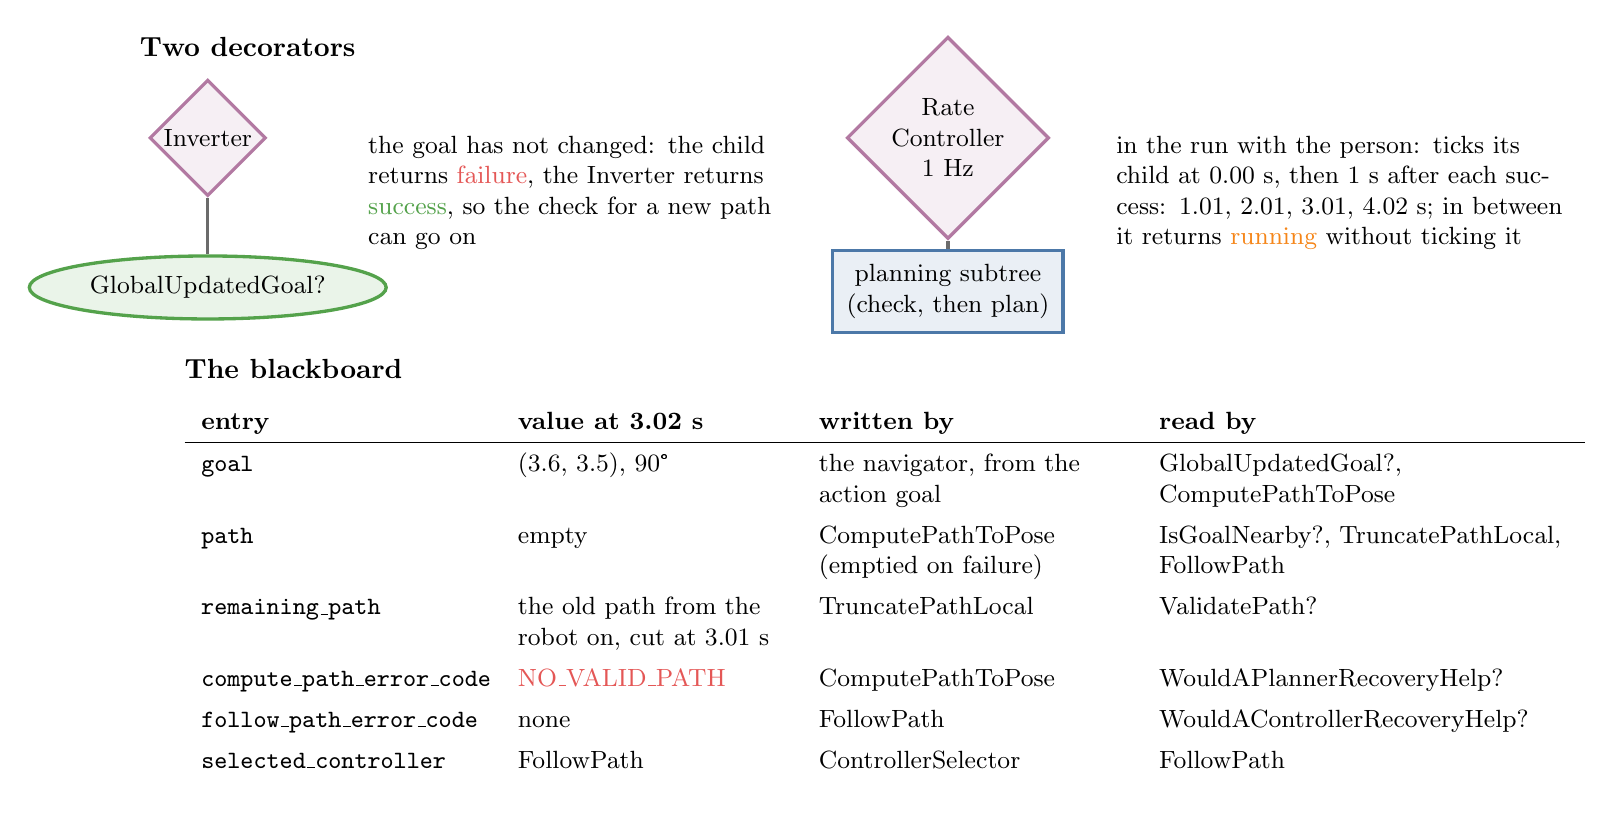
\begin{tikzpicture}[
  dec/.style={diamond, draw=cpurple, fill=cpurple!12, minimum size=1.2cm, inner sep=1pt, font=\small, align=center},
  cnd/.style={ellipse, draw=cgreen, fill=cgreen!12, minimum height=0.8cm, inner sep=3pt, font=\small},
  sub/.style={draw=cblue, fill=cblue!12, minimum height=0.8cm, inner sep=5pt, font=\small, align=center},
  ans/.style={font=\small, align=left, anchor=west},
  edge/.style={draw=cgrey, line width=1.2pt}]
  % Inverter
  \node[dec] (inv) at (0,0) {Inverter};
  \node[cnd] (gug) at (0,-1.9) {GlobalUpdatedGoal?};
  \draw[edge] (inv) -- (gug);
  \node[ans, text width=5.3cm] at (1.9,-0.7) {the goal has not changed: the child returns \textcolor{cred}{failure}, the Inverter returns \textcolor{cgreen}{success}, so the check for a new path can go on};
  % RateController
  \node[dec] (rc) at (9.4,0) {Rate\\Controller\\1 Hz};
  \node[sub] (cp) at (9.4,-1.95) {planning subtree\\(check, then plan)};
  \draw[edge] (rc) -- (cp);
  \node[ans, text width=5.9cm] at (11.4,-0.7) {in the run with the person: ticks its child at 0.00 s, then 1 s after each success: 1.01, 2.01, 3.01, 4.02 s; in between it returns \textcolor{corange}{running} without ticking it};
  % the blackboard
  \node[anchor=north, font=\small] (bb) at (8.6,-3.2) {\renewcommand{\arraystretch}{1.35}%
    \begin{tabular}{>{\raggedright}p{3.6cm} >{\raggedright}p{3.4cm} >{\raggedright}p{3.9cm} >{\raggedright\arraybackslash}p{5.2cm}}
    \textbf{entry} & \textbf{value at 3.02 s} & \textbf{written by} & \textbf{read by}\\ \hline
    \texttt{goal} & (3.6, 3.5), 90\textdegree & the navigator, from the action goal & GlobalUpdatedGoal?, ComputePathToPose\\
    \texttt{path} & empty & ComputePathToPose (emptied on failure) & IsGoalNearby?, TruncatePathLocal, FollowPath\\
    \texttt{remaining\_path} & the old path from the robot on, cut at 3.01 s & TruncatePathLocal & ValidatePath?\\
    \texttt{compute\_path\_error\_code} & \textcolor{cred}{NO\_VALID\_PATH} & ComputePathToPose & WouldAPlannerRecoveryHelp?\\
    \texttt{follow\_path\_error\_code} & none & FollowPath & WouldAControllerRecoveryHelp?\\
    \texttt{selected\_controller} & FollowPath & ControllerSelector & FollowPath\\
    \end{tabular}};
  \node[font=\bfseries, anchor=south west] at (bb.north west) {The blackboard};
  \node[font=\bfseries, anchor=south west] at (-1.0,0.9) {Two decorators};
\end{tikzpicture}
\end{document}
